\documentclass[titlepage, 11 pt]{article}


\usepackage{fullpage}
\usepackage{listings}

\usepackage{amsmath}
\numberwithin{figure}{section}

\usepackage{verbatim}
\usepackage{float}
\usepackage{graphicx}
\graphicspath{{../Figures/}}
\usepackage{setspace}
\usepackage[toc,title,page]{appendix}
\usepackage{pdflscape}
\usepackage{pdfpages}
\usepackage{multirow}

\usepackage{graphicx}
\usepackage{caption}
\usepackage{subcaption}
\usepackage{amssymb}

\usepackage{makecell}

\usepackage{tcolorbox}
\usepackage{enumitem}

\usepackage{hyperref}
\hypersetup{
	colorlinks=true,
	linkcolor=blue,
	filecolor=magenta,
	urlcolor=cyan,
}

\usepackage{array}
\usepackage{colortbl}
\usepackage{lscape}
\usepackage{outlines}

\usepackage[gen]{eurosym}

\usepackage{amsmath}


\usepackage{siunitx}
\usepackage{subcaption}

\usepackage{titling}

\usepackage{multicol}

\usepackage[dvipsnames]{xcolor}

\newcommand{\subtitle}[1]{%
	\posttitle{%
		\par\end{center}
	\begin{center}\large#1\end{center}
	\vskip0.5em}%
	}
	
	
	
	
	\begin{document}


\title{SSA Interpretations}
\author{Environmental Modeling \\ Computational Sciences, AGMETA \\   
	\\ Seed Product Innovation \\ Product Supply  } 

\date{\today}

\maketitle

\tableofcontents
\setcounter{tocdepth}{4}
\newpage

\counterwithin{figure}{section}
\counterwithin{table}{section}


	
	
	\section*{Executive Summary}
	
	Environmental conditions within fields affect the growth of crops in predictable ways. Environmental classification is a process of using environmental features to classify agricultural landscapes into discrete zones that summarize environmental variability that is relevant to crop growth. There is the need to describe macrozones with respect to the features that they contain in order to maximize their utility as management tools.  In particular, SubSahara Africa (hereafter, SSA) utilizes the macrozone model with 25 classes (created by Mike Martinez and Shinichi Kobara), so understanding the variability within and across macrozones also promotes understanding of product segments.  Here, we present initial interpretations of the 25 class macrozone model of SSA along with methodology to facilitate their descriptions.  
	
	
	
	\section*{Macrozones}
	Environmental classification was used to to create 25 discrete zones (called `macrozones') across the entire spatial extent of SSA (Figure 1).  This model was created from a total of 373 features that included three weather features (average maximum temperature, average temperature range, and total precipitation) from 2013 - 2024 with a monthly temporal resolution, day length, also at a monthly temporal resolution, and elevation (Table 1). As result of this analysis, a full description of each macrozone, along with visualization of elevation, climate and day length trends are given in Appendix 1. 
	
	
	
	%Table to describe features
	\begin{table}[H]
		\centering
		\caption{Features used to create the 25 class (macrozone) environmental classification model}  
		\bigskip
		\label{my-label}
		\newcolumntype{P}[1]{>{\centering\arraybackslash}p{#1}}
		\newcolumntype{M}[1]{>{\centering\arraybackslash}m{#1}}
		
		\begin{tabular}{|M{6.0cm} |M{4.5cm}  |M{4.5cm} |}
			\hline
			\multirow{2}{*} {\textbf{Data Layer}} & \multirow{2}{*} {\textbf{Years}}& \multirow{2}{*} {\textbf{Temporal resolution}} \\ 
			\multirow{2}{*} {}                              & \multirow{1}{*}{ }                                            & \multirow{1}{*}{ }      \\ \hline 
			
			\multirow{1}{*} {}                                            & \multirow{1}{*}{ }                                            & \multirow{1}{*}{ }      \\ 
			\multirow{1}{*}{Avg. Max. Temperature}        & \multirow{1}{*}{ }                     & \multirow{1}{*}{ } \\ 
			\multirow{1}{*} {}                                            & \multirow{1}{*}{ }                & \multirow{1}{*}{ } \\  
			
			\multirow{1}{*}{Avg. Temp. Range}                & \multirow{1}{*}{2013 - 2024 } & \multirow{2}{*}{ Monthly }     \\  
			\multirow{1}{*} {}                                            & \multirow{1}{*}{ }                & \multirow{1}{*}{ } \\  
			
			\multirow{1}{*}{Total Precipitation}                & \multirow{1}{*}{ }                 & \multirow{1}{*}{ }  \\ 
			\multirow{1}{*} {}                                            & \multirow{1}{*}{ }                & \multirow{1}{*}{ } \\  \cline{1-2}
			
			
			
			\multirow{2}{*}{Day Length}                  & \multirow{2}{*}{ NA }               & \multirow{1}{*}{  }       \\ 
			\multirow{2}{*} {}                                  & \multirow{1}{*}{ }                     & \multirow{1}{*}{ } \\ \cline{1-3}  
			
			
			\multirow{2}{*}{ Elevation }                 & \multirow{2}{*}{ NA }                        & \multirow{2}{*}{ NA }   \\ 
			\multirow{2}{*} {}                              & \multirow{1}{*}{ }                                 & \multirow{1}{*}{ } \\ \hline
			
			
		\end{tabular}
	\end{table}		
	
	% ------------------------------------------------
	\bigskip	
	
	
	\pagebreak
	
	\begin{center}
		\begin{figure}[H]
			\centering
			
\includegraphics[scale=0.7]{../plots/Macrozones_25.pdf}  
			\caption{Environmental classification of SSA, 25 Macrozones of the 25 class model.    \label{figure:Macrozones_25} }
		\end{figure}
	\end{center}
	
	

	
	
	\newpage
	
	\section*{Results}
	The methodology used to generalize weather trends across macrozones proved to be successful for capturing distinct patterns in weather and day length.  Visualizations of the geographical locations of similar weather patterns across macrozones conform that these distinct trends describe climate shared by distinct macrozones.  Macrozones that share similar climate were further differentiated by differences in day length and elevation.  A full description of each macrozone, along with visualization of elevation, climate and day length trends are given in Appendix 1.
	
	
	\subsection{Daylength}
	
	\begin{center}
		\begin{figure}[H]
			\centering
			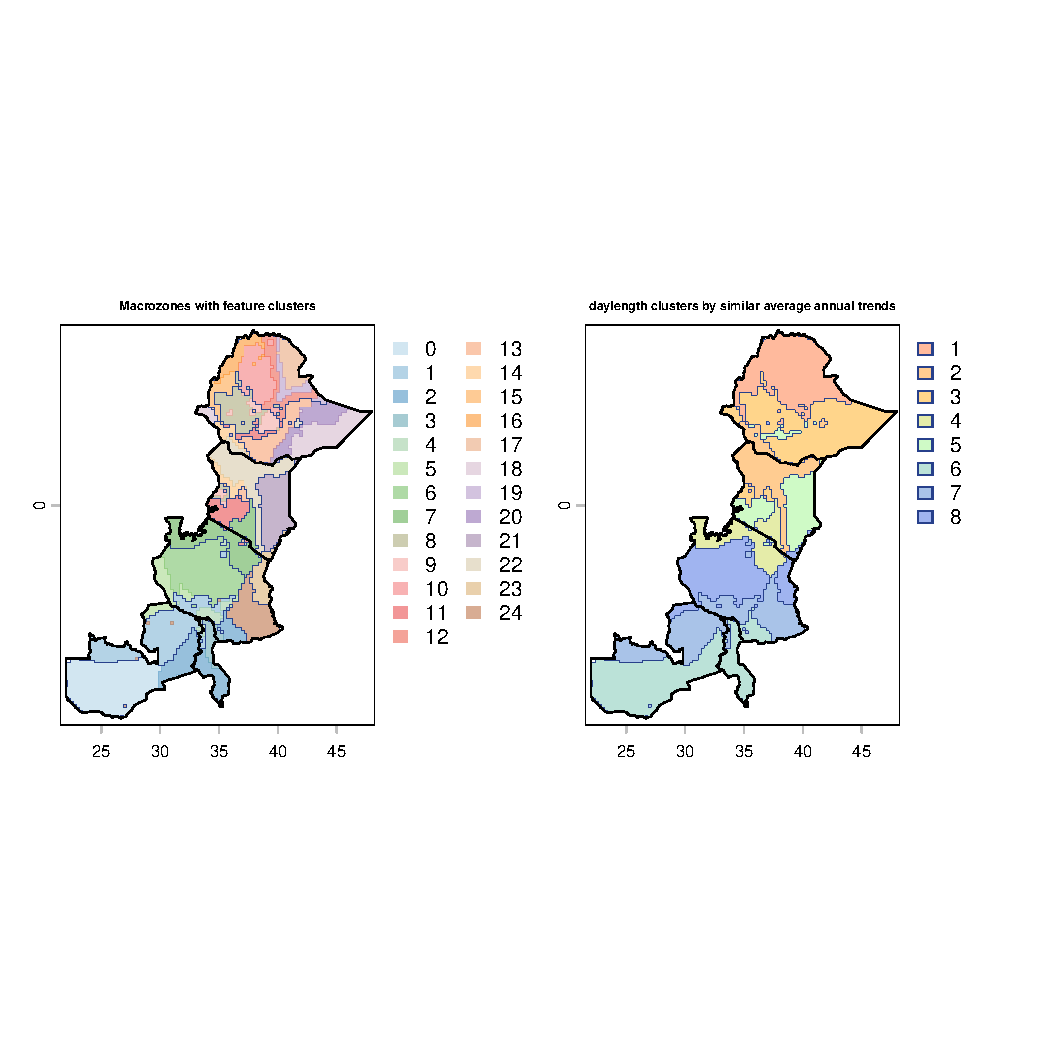
\includegraphics[scale=1]{../plots/feature_cluster_shps/daylength_zones_clusters.pdf}  
			\caption{Daylength clusters.  Clusters group macrozones with similar trends for daylength, by month, throughout the year.    \label{figure:Macrozones_Daylength} }
		\end{figure}
	\end{center}
	
	
	\subsubsection{Daylength summaries across clusters}
	Overview daylength trends across cluster.  Clusters group macrozones with similar trends for daylength, by month, throughout the year.  The lines are average trend per macrozone, colored by macrozone.  The black line is the average for the cluster. 
		
	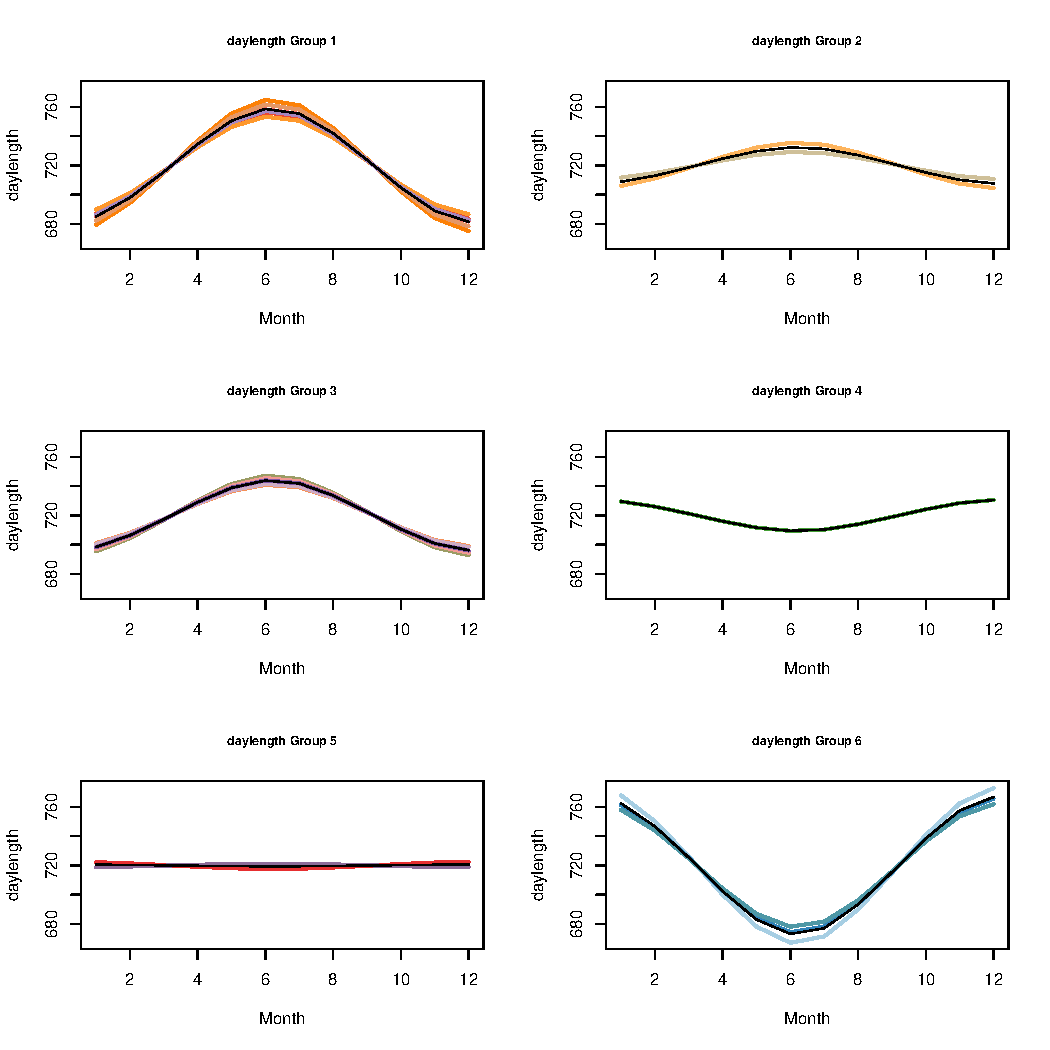
\includepdf[pages=-]{../plots/feature_cluster_trends/daylength_panel.pdf}
	

	\subsubsection{Daylength summaries by cluster}
	Overview daylength trends for each cluster.  Clusters group macrozones with similar trends for daylength, by month, throughout the year.  The lines are average trend per macrozone, colored by macrozone.  The black line is the average for the cluster. 
	
	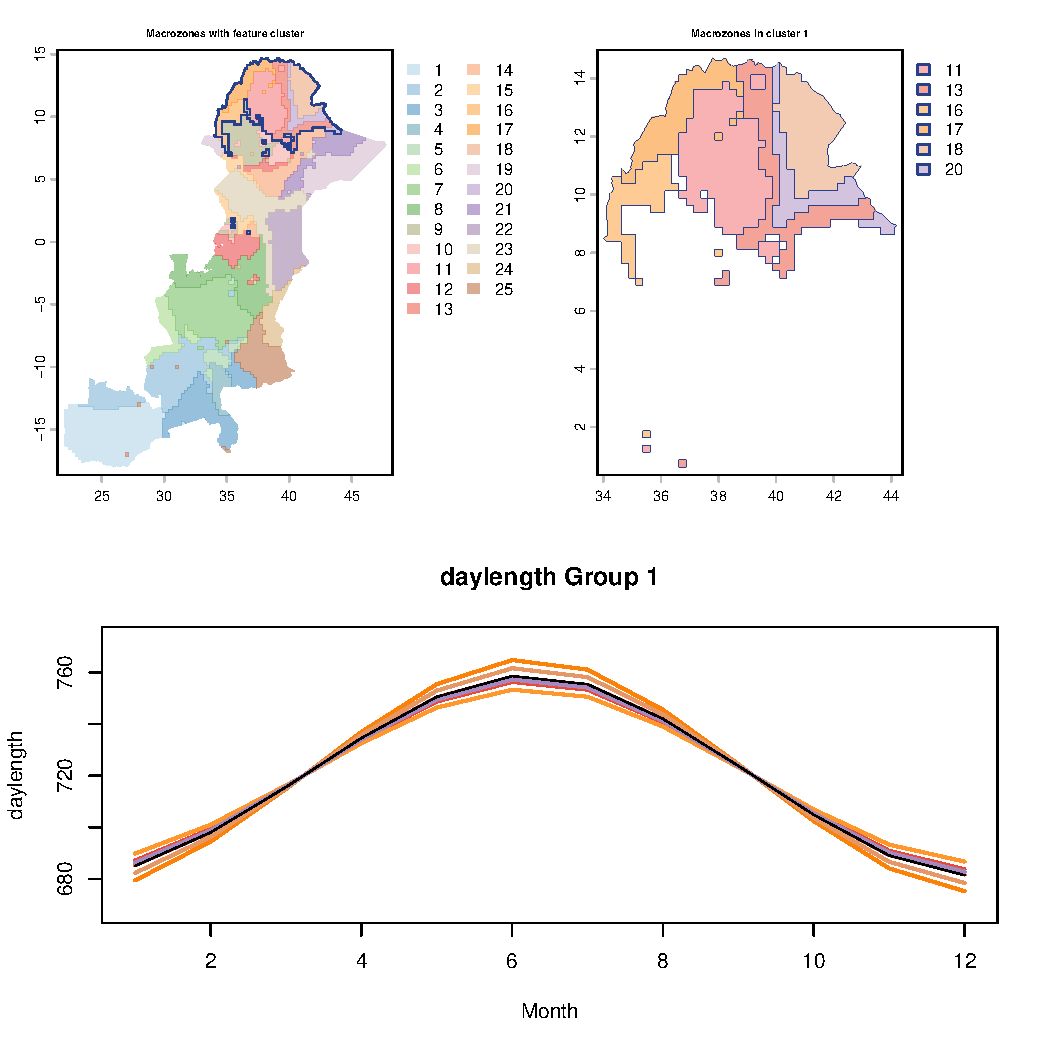
\includepdf[pages=-]{../plots/feature_cluster_trends/daylength_feature_cluster_trend.pdf}
	
	
	
	
	
	
	
	\subsection{Max Temperature}
	
	\begin{center}
		\begin{figure}[H]
			\centering
			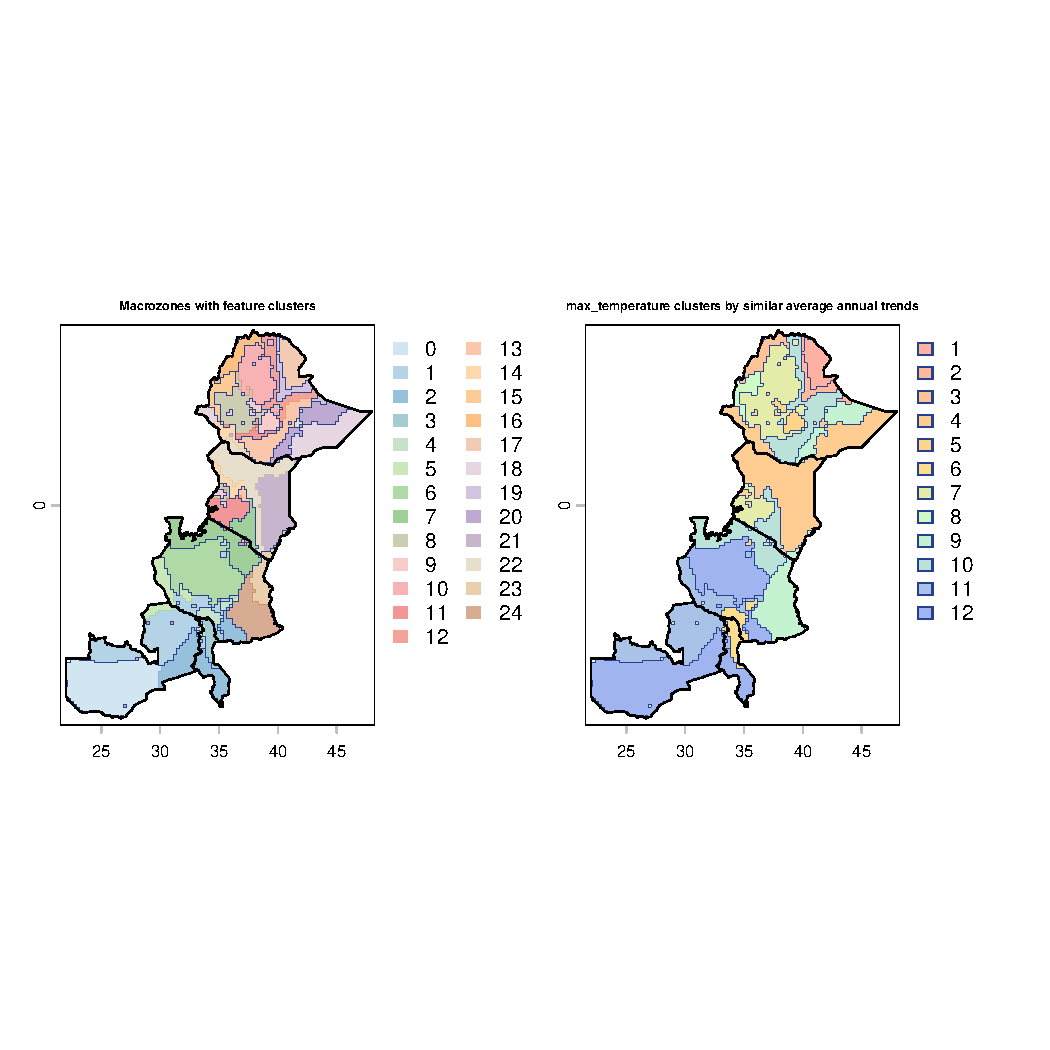
\includegraphics[scale=1]{../plots/feature_cluster_shps/max_temperature_zones_clusters.pdf}  
			\caption{Daylength clusters.  Clusters group macrozones with similar trends for max temperature, by month, throughout the year.    \label{figure:Macrozones_Max_temperature} }
		\end{figure}
	\end{center}
	
	
	\subsubsection{Max Temperature summaries across clusters}
	Overview max temperature trends across cluster.  Clusters group macrozones with similar trends for max temperature, by month, throughout the year.  The lines are average trend per macrozone, colored by macrozone.  The black line is the average for the cluster. 
	
	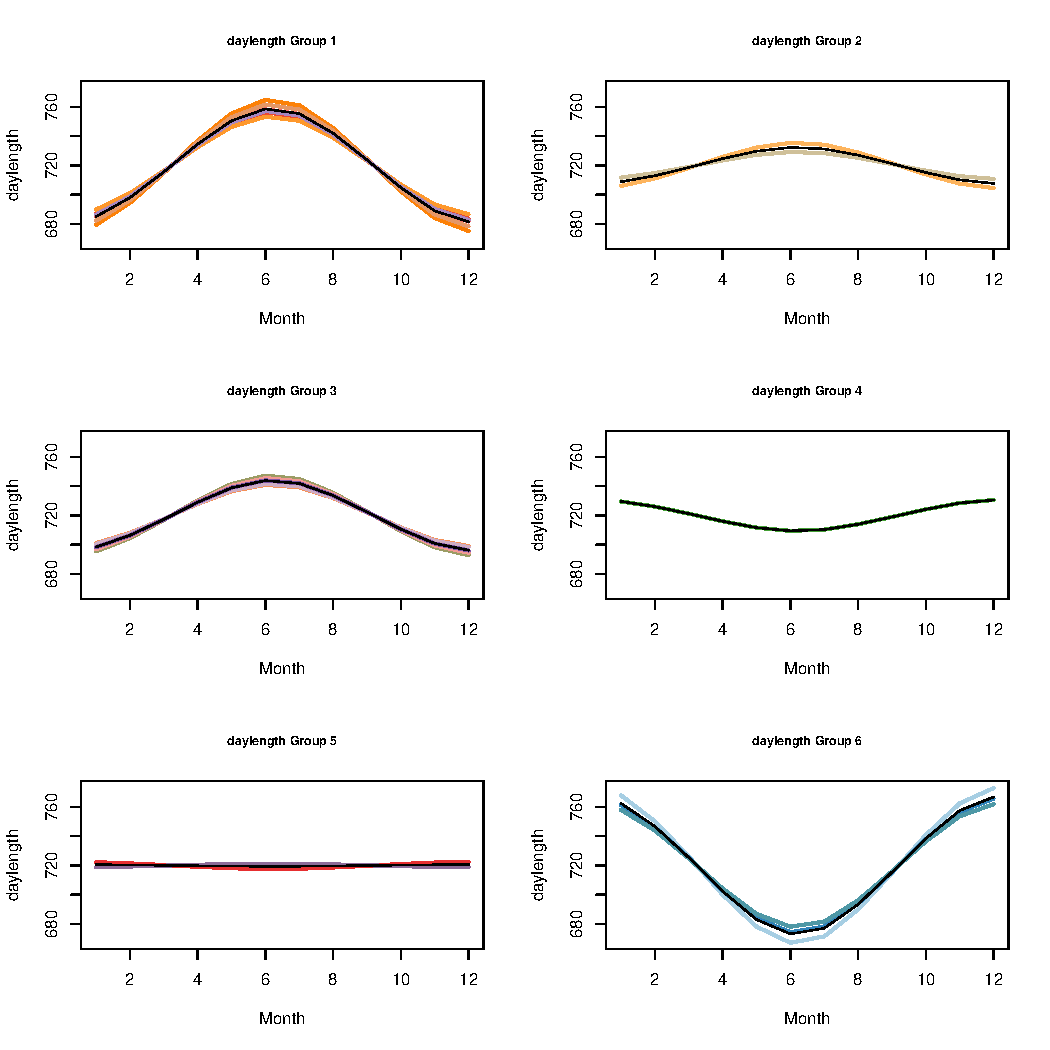
\includepdf[pages=-]{../plots/feature_cluster_trends/daylength_panel.pdf}
	
	
	\subsubsection{Max Temperature summaries by cluster}
	Overview max temperature trends for each cluster.  Clusters group macrozones with similar trends for max temperature, by month, throughout the year.  The lines are average trend per macrozone, colored by macrozone.  The black line is the average for the cluster. 
	
	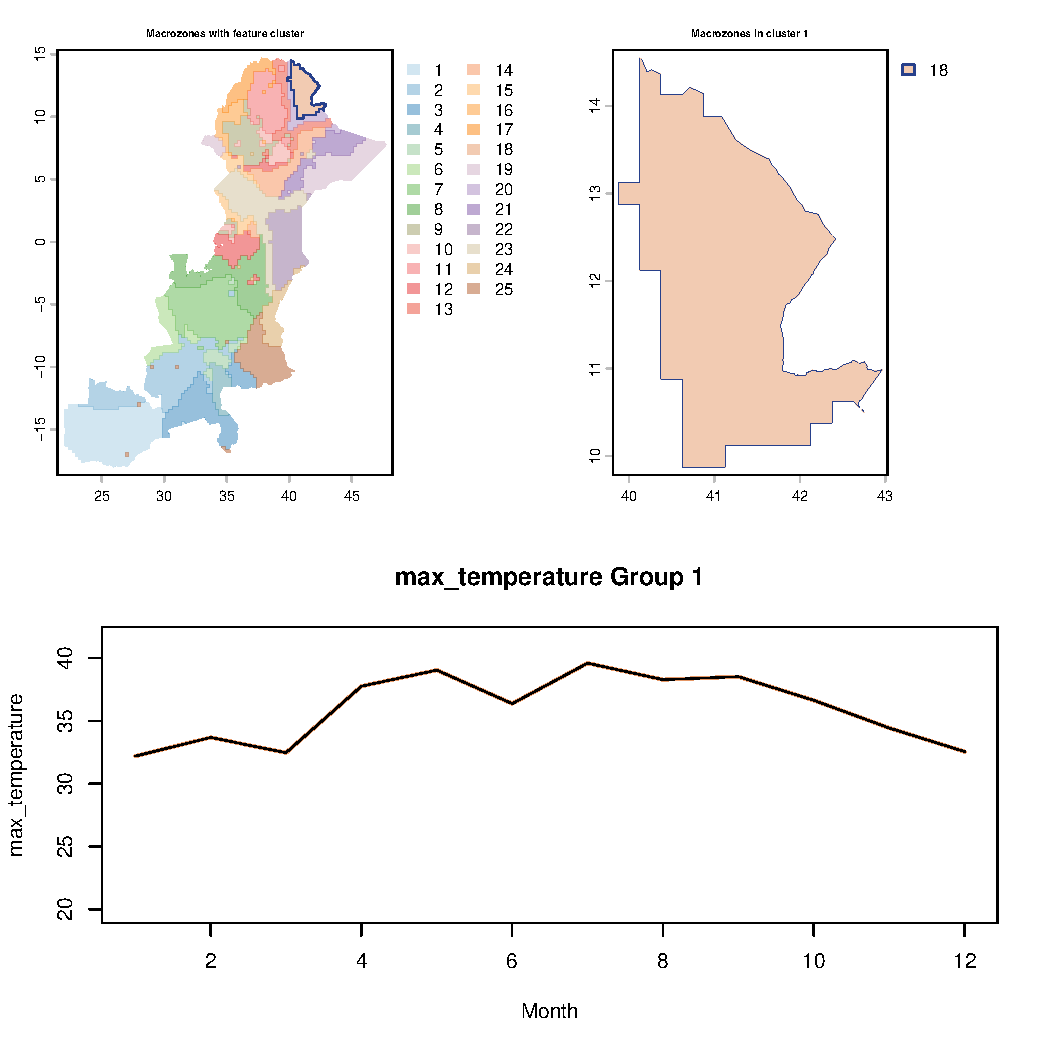
\includepdf[pages=-]{../plots/feature_cluster_trends/max_temperature_feature_cluster_trend.pdf}
	
	
	
	
	
	
	
	
	\subsection{Temperature Range}
	
	
	\begin{center}
		\begin{figure}[H]
			\centering
			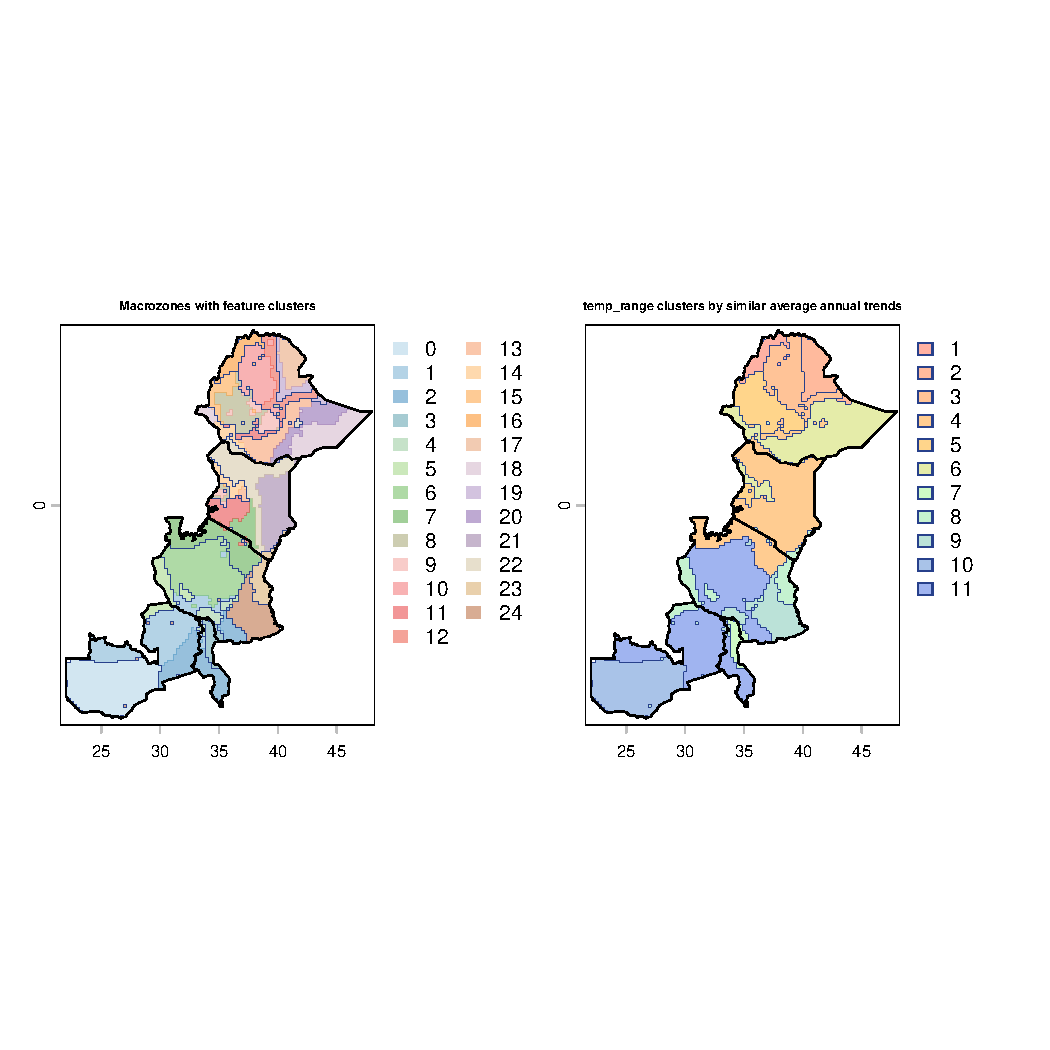
\includegraphics[scale=1]{../plots/feature_cluster_shps/temp_range_zones_clusters.pdf}  
			\caption{Temperature range clusters.  Clusters group macrozones with similar trends for temperature range, by month, throughout the year.    \label{figure:Macrozones_Temperature_range} }
		\end{figure}
	\end{center}
	
	
	\subsubsection{Max Temperature summaries across clusters}
	Overview temperature range trends across cluster.  Clusters group macrozones with similar trends for temperature range, by month, throughout the year.  The lines are average trend per macrozone, colored by macrozone.  The black line is the average for the cluster. 
	
	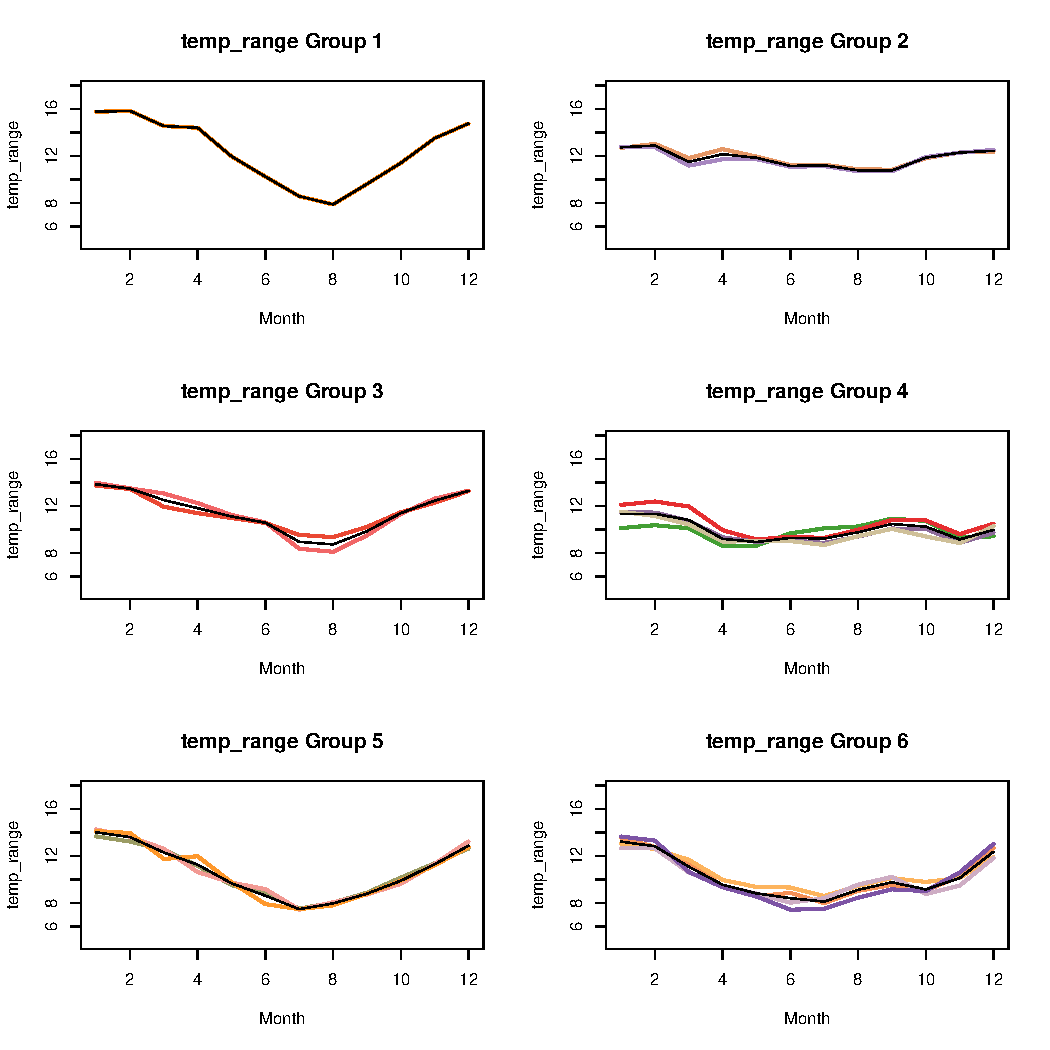
\includepdf[pages=-]{../plots/feature_cluster_trends/temp_range_panel.pdf}
	
	
	\subsubsection{Max Temperature summaries by cluster}
	Overview temperature range trends for each cluster.  Clusters group macrozones with similar trends for temperature range, by month, throughout the year.  The lines are average trend per macrozone, colored by macrozone.  The black line is the average for the cluster. 
	
	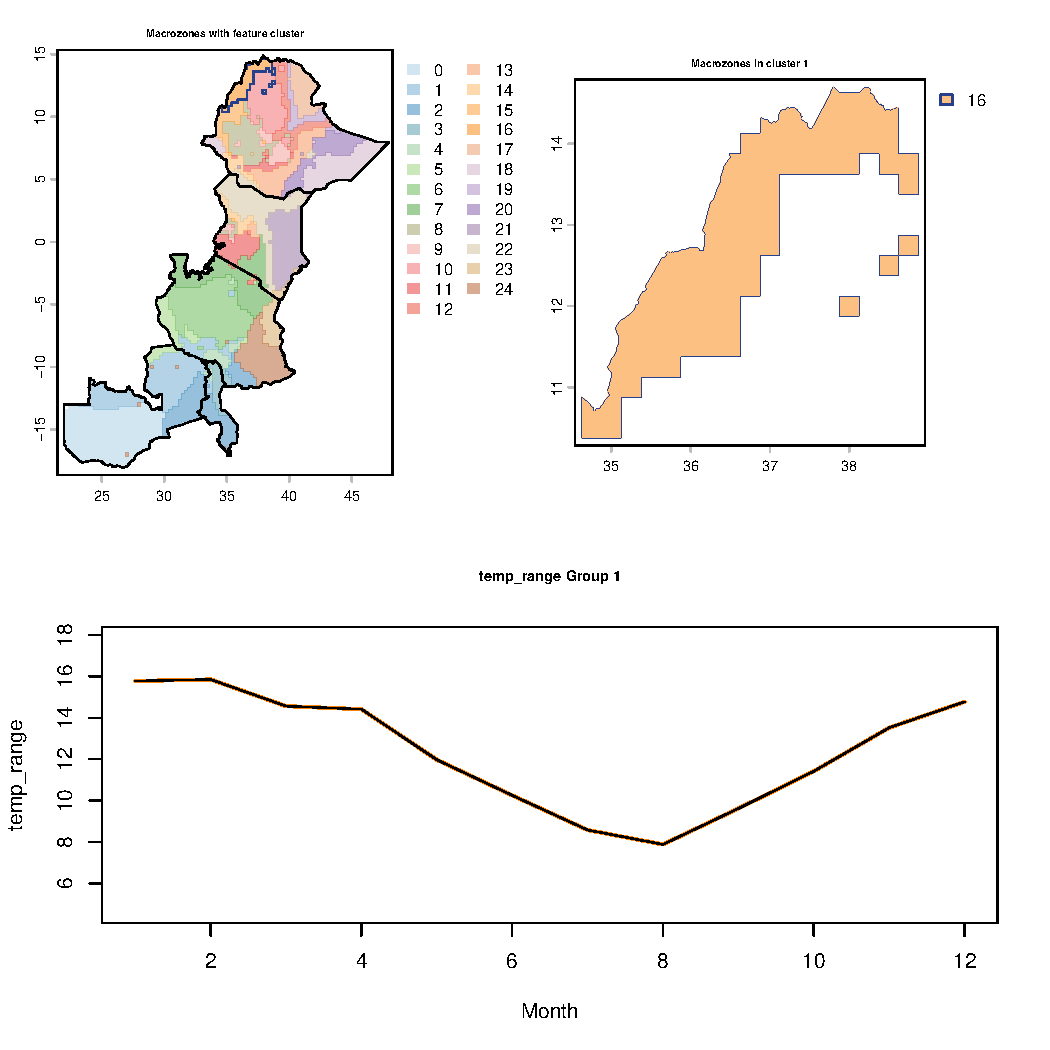
\includepdf[pages=-]{../plots/feature_cluster_trends/temp_range_feature_cluster_trend.pdf}
	
	
	
	
	
	
	
	\subsection{Total Precipitation}
	
	\begin{center}
		\begin{figure}[H]
			\centering
			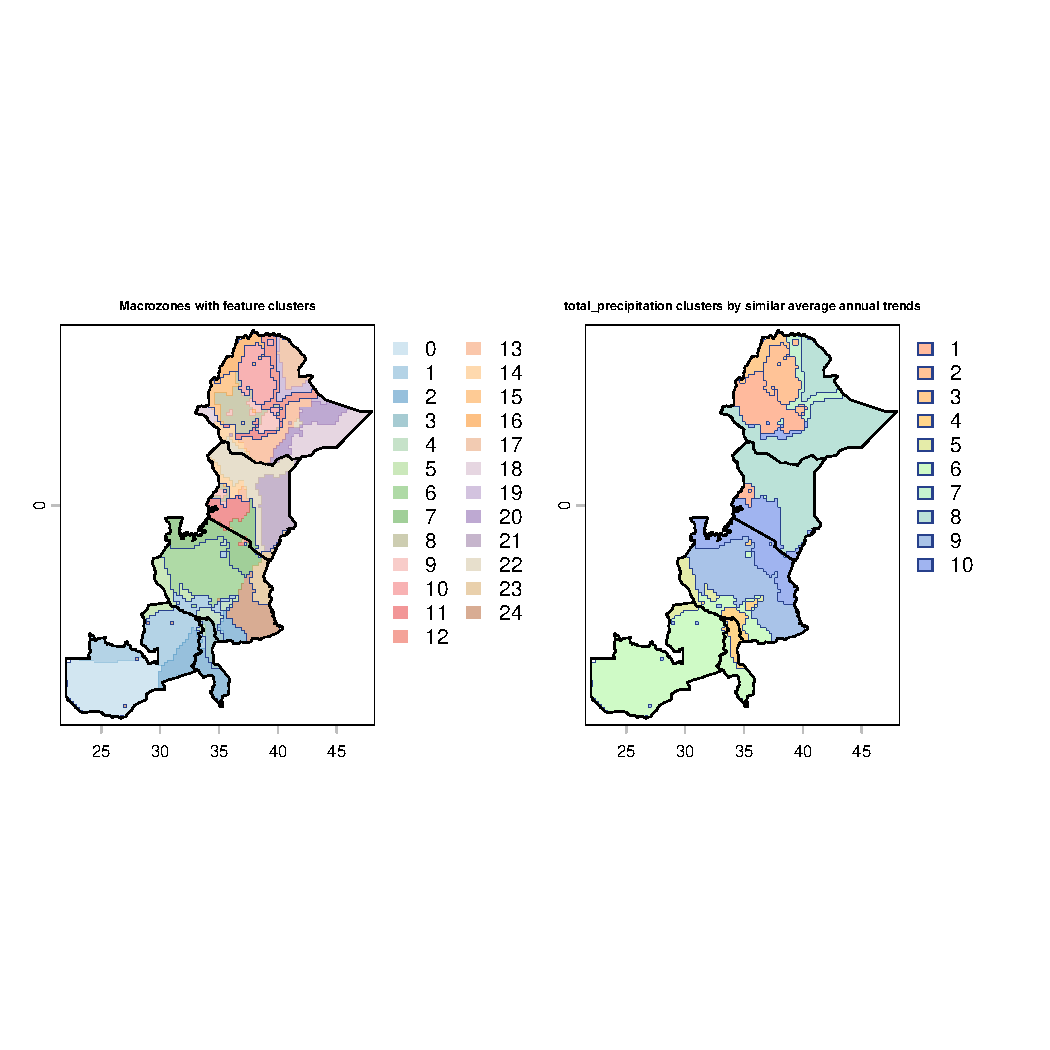
\includegraphics[scale=1]{../plots/feature_cluster_shps/total_precipitation_zones_clusters.pdf}  
			\caption{Temperature range clusters.  Clusters group macrozones with similar trends for total precipitation, by month, throughout the year.    \label{figure:Macrozones_Temperature_range} }
		\end{figure}
	\end{center}
	
	
	\subsubsection{Total Precipitation summaries across clusters}
	Overview temperature range trends across cluster.  Clusters group macrozones with similar trends for total precipitation by month, throughout the year.  The lines are average trend per macrozone, colored by macrozone.  The black line is the average for the cluster. 
	
	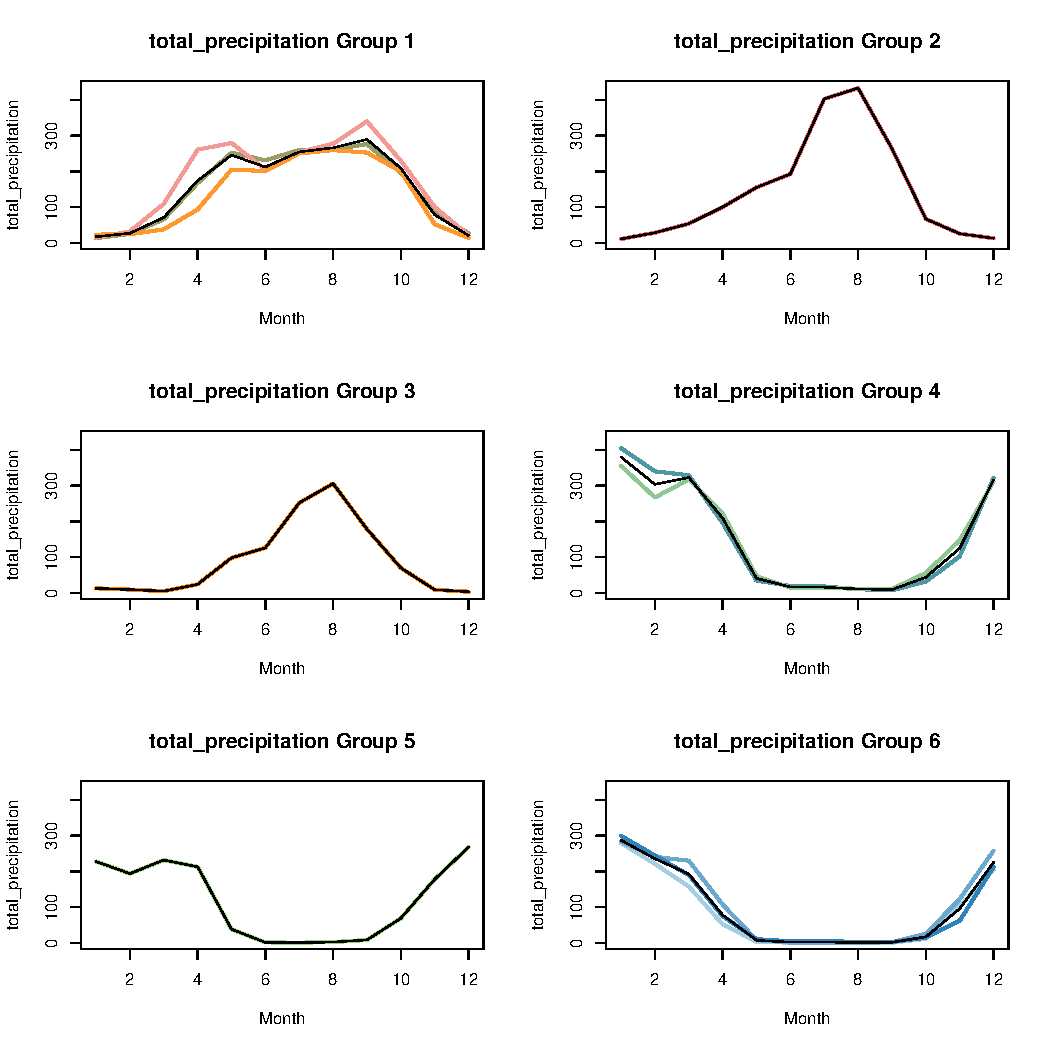
\includepdf[pages=-]{../plots/feature_cluster_trends/total_precipitation_panel.pdf}
	
	
	\subsubsection{Total Precipitation summaries by cluster}
	Overview temperature range trends for each cluster.  Clusters group macrozones with similar trends for total precipitation, by month, throughout the year.  The lines are average trend per macrozone, colored by macrozone.  The black line is the average for the cluster. 
	
	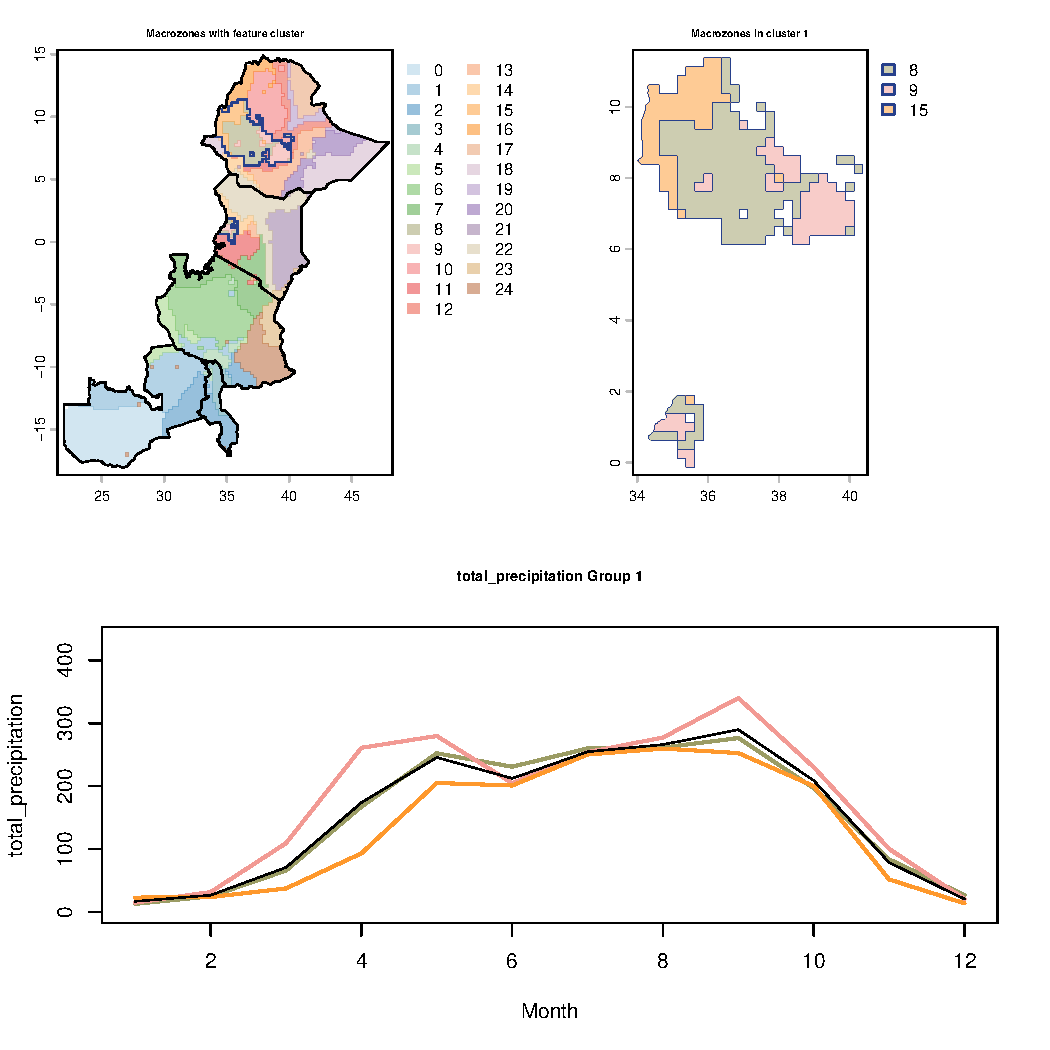
\includepdf[pages=-]{../plots/feature_cluster_trends/total_precipitation_feature_cluster_trend.pdf}
	
	
	
	
	
	
	
	\section*{Materials and Methods}
	One caveat of interpreting macrozones is the high dimensionality of features (here, a 40 X 373 matrix).  The mean and standard deviation of original feature values and feature weights were used to back-transform z-scores of centroids to original values.  These values were used in interpretations.    
	
	\bigskip
	
	\noindent \textbf{Cluster Analysis} \\
	Weather proved to be the most challenging set of features to interpret because each weather feature (average maximum temperature, average temperature range, and total precipitation) was composed of 120 columns (10 years of monthly temporal resolution).  This high dimensionality made it difficult to discern general weather patterns that collective groups of macrozones may have.  We simplified weather trends and observed patterns by performing the following methodology.  For each weather feature, we averaged weather observations for each month within each macrozone to obtain a 10-year average trend at a monthly resolution.  This reduced the total dimensionality to a 40 X 12 matrix containing distinct monthly weather for each macrozone.  
	
	Once average weather was obtained for each macrozone, we wished to compare patterns of weather trends across macrozones.  Ward's clustering was computed on the Euclidean distance of collective average trends for each weather feature.  Scree plots aided the determination of the number of unique weather patterns exhibited across macrozones.  Once the number of clusters were determined, the mean average of annual trends within clusters was calculated and plotted with each separate macrozone weather trend to verify that the approach successfully captured weather patterns.  We performed the same methodology for this day length trend, however day length was already reduced to a single annual trend (a 40 X 12 matrix).  We visualized the new cluster assignments that summarize weather patterns and day length within macrozones by reclassifying macrozone designations to their cluster assignment.  We summarized average elevation within each macrozone with a bar plot.   
	
	
	
	
	
	
	
	
\end{document}	
	